\documentclass[conference]{IEEEtran}
\usepackage{cite}
\usepackage[portuges,brazil]{babel}
\usepackage{amsmath,amssymb,amsfonts}
\usepackage{siunitx}
\usepackage{algorithmic}
\usepackage{graphicx}
\usepackage{textcomp}
\usepackage{hyperref}
\usepackage{listings}
\usepackage[toc,page]{appendix}
\usepackage[utf8]{inputenc}

\def\BibTeX{{\rm B\kern-.05em{\sc i\kern-.025em b}\kern-.08em
    T\kern-.1667em\lower.7ex\hbox{E}\kern-.125emX}}

\begin{document}

\title{Projeto 5: Compressão de imagens por SDV\\
\large .\\
\large MC920 - Introdução ao Processamento Digital de Imagem (MC920 / MO443) 2S2019\\
\large Professor: Hélio Pedrini}

\newcommand{\email}[1]{\href{mailto:#1}{#1}}

\author{
    \IEEEauthorblockN{Giovani Nascimento Pereira}
    \IEEEauthorblockA{
    \email{giovani.x.pereira@gmail.com} \\
    168609
    }
}

\maketitle

\section{Definição do problema}

    SDV, ou \textit{Single Value Decomposition}, aplicado ao contexto de processamento de imagens, é uma técnica de compressão baseada na projeção de dados em subespaços.

    \subsection{Objetivo}

        O objetivo deste trabalho é de implementar a técnica de compressão SDV para imagens coloridas e depois analisar esse resultado.

    \subsection{Execução do projeto}

        Para executar o script do projeto \textit{main.py} são utilizados os comandos:

        \begin{lstlisting}[language=bash]
        $ python3 main.py [input_path]
        [-k valor] [-o output_path]
        \end{lstlisting}

        Onde:

        \begin{itemize}
            \item \textit{input\_path} é o caminho da imagem de entrada
            \item \textit{-k valor} é o valor $k$ do nível de compressão
            \item \textit{-o output\_path} é o caminho para salvar a imagem de saída (o caminha padrão é \textit{./compressed.png}).
        \end{itemize}

        A imagem de entrada esperado é colorida e no formato PNG. A imagem gerada de saída também estará no formato PNG por padrão.

        Um menu de ajuda pode ser exibido através do comando:

        \begin{lstlisting}[language=bash]
        $ python3 main.py --help
        \end{lstlisting}

\section{Resultados}

    A partir do script gerado para compressão SDV, foi aplicado a compressão para diversos valores de $k$ utilizando uma das imagens de entrada fornecidas para o experimento.
    A imagem escolhida foi a do \textit{baboon.png} e o resultado pode ser observado na figura \ref{compressed_monkey}.

    \begin{figure}[htb]
        \centering
        \includegraphics[width=\linewidth]{compressed_monkey.png}
        \caption{Resultados de compressão SDV aplicados à imagem do \textit{baboon.png}, (a) imagem original, (b) k = 2, (c) k = 5, (d) k = 10, (e) k = 25, (f) k = 50, (g) k = 75, (h) k = 100}
        \label{compressed_monkey}
    \end{figure}

    Também para compreender como a taxa de compressão funcionou em cada conjunto de imagens, foi calculado $p$, taxa de compressão, através da expressão \ref{p}.

    \begin{equation}
        p = \dfrac{\text{quantidade de memória para representar g}}{\text{quantidade de memória para represemtar f}}
    \end{equation}

    Onde g é a imagem comprimida e f e imagem original.

    Com isso, podemos montar uma tabela que exibe os resultados entre o fator de compressão e o fator $k$ utilizado, tabela \ref{p}.

    \begin{table}[]
\begin{tabular}{|l|l|l|l|}
\hline
\textbf{k} & \textbf{\begin{tabular}[c]{@{}l@{}}Memória para\\ armazenamento (Kb)\end{tabular}} & \textbf{Fator de compressão ($p$)} & \textbf{RMSE} \\ \hline
-          & 637.19                                                                             & 1                                  & 0             \\ \hline
2          & 217.92                                                                             & 0.342                              & 44.295        \\ \hline
10         & 352.22                                                                             & 0.552                              & 29.291        \\ \hline
20         & 420.73                                                                             & 0.660                              & 26.965        \\ \hline
25         & 445.98                                                                             & 0.699                              & 26.015        \\ \hline
50         & 516.01                                                                             & 0.809                              & 22.302        \\ \hline
75         & 553.80                                                                             & 0.869                              & 19.581        \\ \hline
100        & 577.14                                                                             & 0.906                              & 17.212        \\ \hline
\end{tabular}
    \caption{Memória necessária para armazenar as imagens comprimidas, erro médio quadrático e fator de compressão para diferentes $k$}
    \label{p}
    \end{table}

    Para compreender melhor como  a compressão afetava cada canal de cor, para um valor fixo de $k = 5$, foi também gerada as imagens de cada canal de cor individualmente em escalas de cinza. O resultado pode ser observado na figura \ref{channel_monkey}

    \begin{figure}
        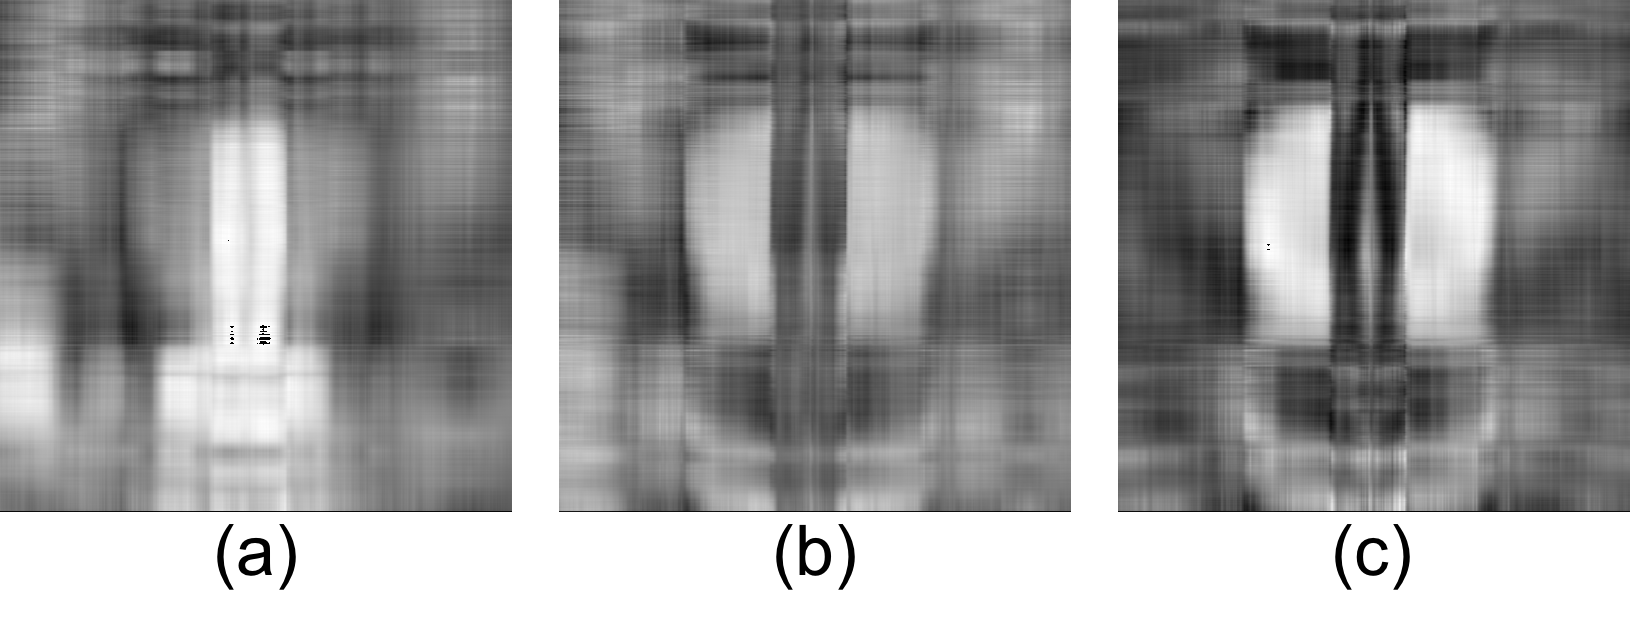
\includegraphics[width=\linewidth]{channel_monkey.png}
        \caption{Resultados da compressão da imagem do \textit{baboon.png} para um fator $k=5$ observando o resultado em cada canal de cor individualmente. (a) cor vermelha, (b) cor verde, (c) cor azul}
        \label{channel_monkey}
    \end{figure}


\section{Análises}

    Se observarmos as imagens da figura \ref{compressed_monkey}, podemos notar que quão maior o fator $k$, mais próxima da imagem original estará a imagem comprimida, mas que também assim é menor o grau de compressão da imagem.

    A imagem tratada em questão tinha formato $512$x$512$ pixels, e para valores muito pequenos de $k$ como $2$ ou $5$, ali representados, é difícil perceber do que se trata a imagem como um todo.

    Um ponto importante da compressão SDV é que ela introduz perdas ao conjunto da imagem, consegue reduzir o erspaço de memória necessário para armazenamento, mas com isso parte das informações da imagem são perdidas.
    Então, apesar de ser uma técnica interessante para a redução da memória de armezenamento, não pode ser aplicada em toda situação.

    Se observarmos os resultados da tabela \ref{p} é possível notar que o método de compressão foi efetivo em reduzir o tamanho do espaço de memória necessário para o armazenamento da imagem, e conforme o fator $k$ dominui, diminui a qualidade da imagem em relação à original e também a memória necessária para o armazenamento.

    A diferença entre a imagem comprimida ee a original, tembám está exporessa na tabela \ref{p}, na coluna RMSE, que representa o erro quadrático médio.
    E nesse caso, o erro é maior quanto menor o fator $p$, o que já era esperado dado que a qualidade da imagem são as que mais se distinguem da imagem original.


    Agora, podemos analisar a imagem \ref{channel_monkey}, que mostra a compressão aplicada a cada canal de cor individualmente. É interessante perceber que apesar da compressão ser a mesma nos 3 canais da imagem colorida, os resultados visuais são diferentes pois cada canal possui uma sequência de níveis de cinza diferente.


\section{Conclusão}

    Através dos resultados obtidos no projeto, é possível notar que o comportamento encontrado foi satisfatório.
    As imagens comprimidas tem comportamento semelhante ao esperado na literatura e também foi possível observar a compressão em cada canal de cor individualmente.

    Analisando os valores de $p$ e $RMSE$ é possível ter uma noção que para valores próximos de $k = 100$, a quantidade de perda da imagem é pequena, ou seja tem um RMSE baixo, então poderia ser uma técnica empregada para a redução de qualidade das foto, desde que seja permitido a perda de informações dentro da imagem.

\begin{thebibliography}{00}

  \bibitem{helio} Helio Pedrini. Trabalho 5. Introdução ao Processamento Digital de Imagem (MC920 / MO443), 2019.\\

  \bibitem{srgb} SRGB. disponível em \url{https://en.wikipedia.org/wiki/SRGB}. Acesso 11 de setembro de 2019.

\end{thebibliography}

\end{document}
